\chapter{Executive Summary}

In this penetration test, the provided VM by the lecturer was assessed for security vulnerabilities. 
The assessment was conducted between the 18th February and the 18th March as a black box test, 
thus, no specific information about the internals of the system were provided. The scope of the assessment was as follows:
\begin{itemize}
	\item Virtual Machine: 10.1.0.10
\end{itemize}
As a result, several vulnerabilities have been identified among the assets of the VM, some of which pose a significant risk.
We found a few services running on the machine, which makes it vulnerable to exterior threats.
Two of these vulnerabilities \ref{weak_password} and \ref{management_server} are highly critical and allow an adversary to gain full access to the VM with all permissions, 
which would have a severe impact on the system. 
The solutions to these two vulnerabilities are not complicated and should be the top priority.

Other threats can be mitigated easily by keeping the system up to date and taking services offline that are not in use.
Therefore, we recommend reviewing the services you need to run on this machine.
Unnecessary services should be turned off, and the ones kept should be updated to the newest version. 

Solutions to remedy the discovered vulnerabilities are provided together with detailed descriptions and reproduction steps in chapter 3.

\begin{figure}[h]
	\centering
	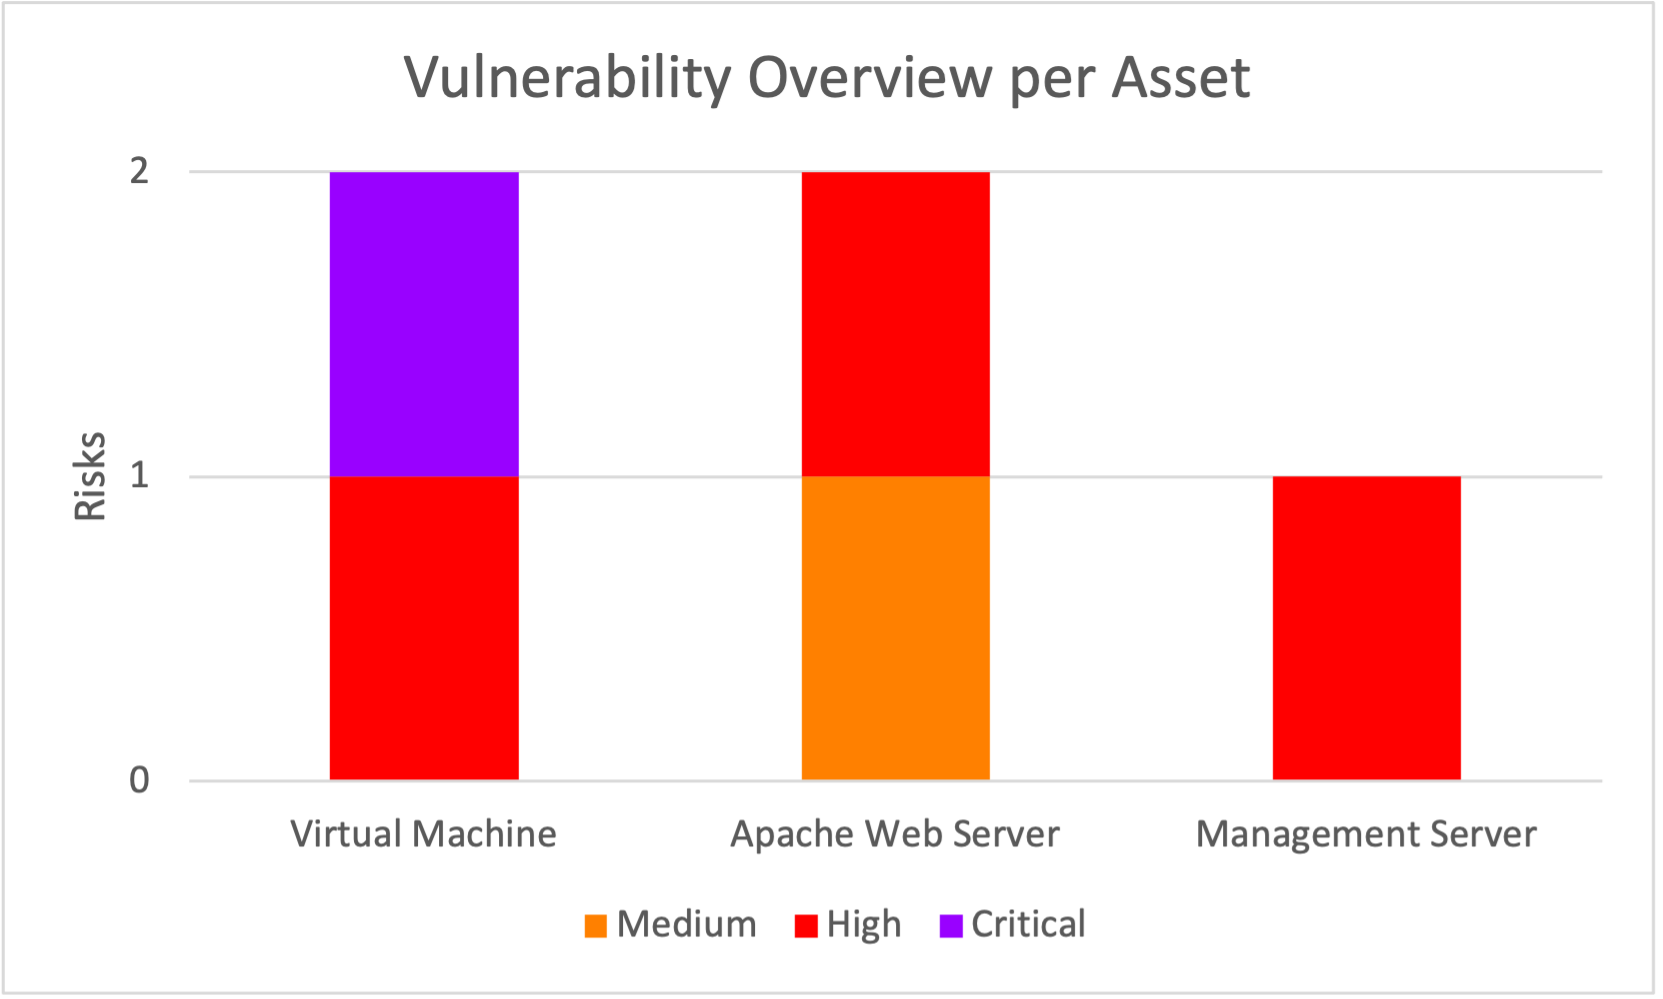
\includegraphics[width=13.5cm]{img/vuln_chart.png}
	\caption{Vulnerability Overview}
\end{figure}
	